\documentclass[12pt, a4paper]{report}
\linespread{1.3}
\setlength{\parindent}{1.25cm}

\usepackage[top=3cm,left=3cm,right=2cm,bottom=2cm]{geometry}
\usepackage{indentfirst}
\usepackage{amsmath, amsthm, amsfonts, amssymb}

\usepackage{graphicx}
\usepackage{color}
\usepackage{multicol}
\usepackage[normalem]{ulem}
\usepackage{wrapfig}
\usepackage{caption}
\usepackage{fancybox}
\usepackage[pdfstartview=FitH]{hyperref}
\usepackage{subfigure}

\usepackage[T1]{fontenc}		% Selecao de codigos de fonte.
\usepackage[utf8]{inputenc}
\usepackage[brazil]{babel}

\usepackage{array}
\usepackage{longtable}
\usepackage{pdfpages}

\usepackage{verbatim}
\usepackage{enumitem}          % criação de linhas

%Includes "References" in the table of contents
\usepackage[nottoc]{tocbibind}

\graphicspath{{Figuras/}} % caminho padrao imagens
% ------ Remove nome capitulo da tag chapter ---------
\makeatletter
\def\@makechapterhead#1{%
  \vspace*{0\p@}%
  {\parindent \z@ \raggedright \normalfont
    \interlinepenalty\@M
    \Huge\bfseries  \thechapter.\quad #1\par\nobreak
    \vskip 30\p@
  }}
\makeatother
\begin{document}

%---------- CAPA -------------

\begin{figure}[ht]
\centering

\includegraphics[scale=0.15]{UFBA.jpg}
\end{figure}

\begin{center}
\sc{\large{Universidade Federal da Bahia - UFBA}} \\
\sc{\large{Instituto de Matematica - IM}} \\
\sc{\large{Departamento de Ciência da Computação - DCC}} \\
\sc{\small{Bacharelado em Sistemas de Informação - BSI}} \\
\sc{\small{Trabalho de Conclusão de Curso}} \\

\vspace{4cm}

\sc{\Large{Desenvolvimento e Avaliação\\do SICAD - UFBA}}

\vspace{4.5cm}

\sc{\Large{Kênia Arruda Guimarães}}

\vspace{5.5cm}

\textbf{Salvador - Bahia} \\
Dezembro de 2019

\end{center}

%---------- FOLHA DE ROSTO -------------
\newpage
\begin{center}
\sc{\Large{Desenvolvimento e Avaliação\\do SICAD - UFBA}}

\vspace{4cm}

\large{Kênia Arruda Guimarães}
\end{center}

\vspace{4cm}

\begin{flushright}
\begin{minipage}{8.6cm}
Monografia apresentada como trabalho de conclusão de curso para o curso de Bacharelado em Sistemas de Informação do Departamento de Ciência da Computação na Universidade Federal da Bahia.

\vspace{0.5cm}
\textbf{Orientador}: Prof. Dr. Rodrigo Rocha Gomes e Souza.

\end{minipage}
\end{flushright}
 
\vspace{8cm}


\begin{center}
\textbf{Salvador - Bahia} \\
Dezembro de 2019
\end{center}

\presentationpage

%%%%%%%%%%%%%%%%%%%%%%
% Ficha Catalográfica
\newpage
\thispagestyle{empty}
\null\vfill
                  
\begin{center}
 Ficha catalográfica.
\begin{tabular}{|p{13.5cm}|}%{p{12cm}}
\hline
\begin{small}
\begin{verbatim}
Guimarães, Kênia Arruda
Desenvolvimento e Avaliação do SICAD-UFBA. / Kênia
Arruda Guimarães. - Salvador, 01, 2008.

182p.:il.
Orientador: Rodrigo Rocha Gomes e Souza.

Monagrafia (Graduaçao) -UNIVERSIDADE FEDERAL DA BAHIA,
INSTITUTO DE MATEMÁTICA, 06 de abril de 2017.

TOPICOS PARA FICHA CATALOGRAFICA.I. 
Souza, Rodrigo Rocha Gomes e. II. UNIVERSIDADE FEDERAL DA BAHIA. 
INSTITUTO DE MATEMÁTICA. III Título.
                                                  NUMERO CDD
\end{verbatim}
\end{small}
\\ \hline
\end{tabular}
\end{center}
\setcounter{page}{2} %truque para não numerar a página


%---------- BANCA EXAMINADORA -------------
\newpage
\begin{center}
\sc{\Large{Desenvolvimento e Avaliação\\do SICAD - UFBA}}

\vspace{2.2cm}

\large{Kênia Arruda Guimarães}
\end{center}

\vspace{2.2cm}

\begin{flushright}
\begin{minipage}{8.6cm} 
Monografia apresentada como trabalho de conclusão de curso para o curso de Bacharelado em Sistemas de Informação do Departamento de Ciência da Computação na Universidade Federal da Bahia.
\end{minipage}
\end{flushright}
 
\vspace{1cm}
\begin{center}
\Large \textbf{Banca Examinadora:}
\end{center}
\vspace{1.5cm}

\begin{flushright}
\begin{minipage}[l]{12cm}
\begin{center}
\uline{\hspace{10.5cm}} \\
Prof. Dr. Rodrigo Rocha Gomes e Souza (Orientador) \\ Universidade Federal da Bahia \\
\vspace{1cm}
\uline{\hspace{10.5cm}} \\

\vspace{1cm}
\uline{\hspace{10.5cm}} \\


\end{center}
\end{minipage}
\end{flushright}

%-----------Dedicatória----------------
\newpage
\vspace*{21cm}
\begin{flushright}
\textit{Dedico este trabalho à minha família}
\end{flushright}


%------------Agradecimentos------------
\newpage
\chapter*{Agradecimentos}
\thispagestyle{empty}
\par Aos meus pais que sempre estiveram ao meu lado me apoiando em cada decisão tomada. À minha noiva Juliana Alves Pereira que vem sendo meu maior suporte neste ciclo de aprendizado. À minha amiga Lina Mendes que me deu grande auxílio no design da aplicação. Aos meus amigos e em especial a Carlos Henrique e Ludmila Cruz que sempre tiveram muita paciência ao ouvir os desabafos quando ainda não tinha encontrado a solução para alguns dos obstáculos que encontrei durante a a execução deste projeto. E por fim, ao meu orientador Rodrigo Rocha Gomes e Souza pela excelente orientação, paciência e atenção prestados no desenvolvimento deste trabalho e a Universidade Federal da Bahia (UFBA) pelo espaço público de ensino que mesmo com todas as dificuldades encontradas forma profissionais excelentes que trarão conhecimento contribuindo para o desenvolvimento do nosso país.  

%------------Citação-------------------
\newpage
\vspace*{20cm}
\begin{flushright}
\begin{minipage}{7cm}
\begin{flushright}
\textit{
"Toda a ciência é nada mais do que um refinamento do pensamento cotidiano". \\
Albert Einstein}
\end{flushright}
\end{minipage}
\end{flushright}


%--------------Resumo-------------------
\newpage
\chapter*{Resumo}
\thispagestyle{empty}


%-------------Abstract------------------
\newpage
\chapter*{Abstract}
\thispagestyle{empty}

%-------------Índice--------------------
\newpage
\tableofcontents
\thispagestyle{empty}

% ----------- Lista de figuras ----------

\pdfbookmark[0]{\listfigurename}{lof}
\listoffigures
\cleardoublepage

%--------- Lista de tabelas ---------

\pdfbookmark[0]{\listtablename}{lot}
\listoftables
\cleardoublepage

%-------------Capítulo 1-----------------
\chapter{Introdução}

%-------------Capítulo 2-----------------
\chapter {Trabalhos Relacionados}

%-------------Capítulo 3-----------------
\chapter{Solução Proposta: SICAD}
\par Como solução para a problemática apresentada neste trabalho, está sendo proposto o Sistema Colaborativo de Avaliação Docente, SICAD, como ferramenta auxiliar para os discentes da Universidade Federal da Bahia utilizarem, a fim de disponibilizar feedbacks e avaliações sobre as disciplinas cursadas. 
\par O processo de concepção do SICAD foi realizado inicialmente como uma junção do trabalho já realizado pelo Sistema de Avaliação Docente, o SIAV\footnote{SIAV. Disponível em <\url{www.siav.ufba.br/siav/privado/index.faces}>. Acesso em: 11 nov. 2019.} disponibilizado pela UFBA\footnote{UFBA. Disponível em <\url{www.ufba.br}> . Acesso em: 1 nov. 2019.} com uma funcionalidade de se realizar comentários, que será especificada no subtópico a seguir. A partir deste escopo foram traçados os requisitos da solução que serão descritos abaixo.

\section{ Modelo Conceitual}
\par 
Por definição \textbf{modelo conceitual} é um conjunto de suposições baseadas no mundo real que indicarão as regas de negócio de um sistema\cite{mapaconceitual}.
\par A importância do desenvolvimento de um mapa conceitual no contexto deste trabalho é a representação gráfica do modelo proposto, referente os processos utilizados na utilização do SICAD, a fim de que ele possa ser entendido de forma fluída.
\par Existem três macros processos   

\section{ Autenticação}
\par Inicialmente foi pensado em um login básico para autenticação no sistema. Contudo, analisando o contexto, o cenário abrangeria qualquer usuário logado na internet que possuísse o caminho do sistema, não sendo interessante pois os mesmos teriam acesso a resultados que possuem informações sensíveis.
\par Para delimitar o acesso ao SICAD, foi utilizado o módulo de \href{https://www.autenticacao.ufba.br}{autenticação} disponibilizado pela UFBA. Sua utilização segue o seguinte processo: a aplicação no momento do login, faz uma requisição à autenticação e a mesma retorna o username \footnote{Username. Disponível em <\url{www.cartilha.cert.br/senhas/}> . Acesso em: 1 nov. 2019.} caso o usuário possua cadastro na universidade. Segue abaixo o fluxograma do processo.
\begin{figure}[!ht]
\centering
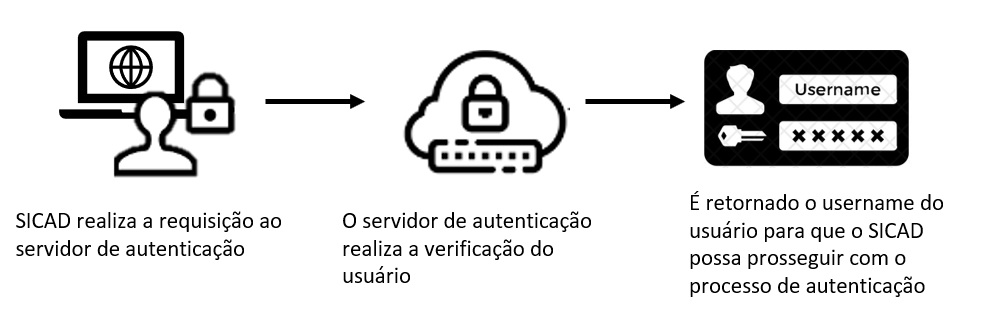
\includegraphics[scale=0.50]{processo_autenticacao.jpg}
\caption{Fluxograma da Requisição de Autenticação}
\label{fig:processo_autenticacao}
\end{figure}

\par Dessa forma o acesso fica restrito a quem possuí cadastro na universidade não expondo assim informações indevidas a usuário que não são elegíveis para utilizar o SICAD.

\subsection{Usuário e Segurança}
\par No processo de desenvolvimento  da autenticação ficou claro a necessidade da implementação de uma camada de segurança, visto que a resposta à requisição feita juntamente a UFBA retorna o username do usuário sem nenhum tipo proteção.
\par A segurança da informação é essencial no sentido de preservar o valor dessa informação que é chave para a maioria das funcionalidades do SICAD. Focando neste ponto foram implementadas rotinas para prover segurança nos processos executados pelo sistema que será descrito nos passos abaixo:

\begin{itemize}
\item o usuário tenta logar no sistema, consequentemente disparando uma requisição para a autenticação da UFBA;
\item A UFBA executa todas as rotinas de validação.
Caso se obtenha uma resposta positiva, retorna o username do usuário sem criptografia para a aplicação que solicitou a requisição;
\item O SICAD antes de persistir a informação no banco de dados, utiliza da tecnologia de criptografia Hash SHA256\footnote{Hash SHA256. Disponível em <\url{www.tsapps.nist.gov/publication/get_pdf.cfm?pub_id=910977}> . Acesso em: 2 nov. 2019.}, que será abordada no tópico 3.6. para encriptografar o username que será chave para utilização do sistema.
\end{itemize}
\par Para melhor fixação segue uma imagem com o fluxo do processo.
\begin{figure}[ht]
\centering
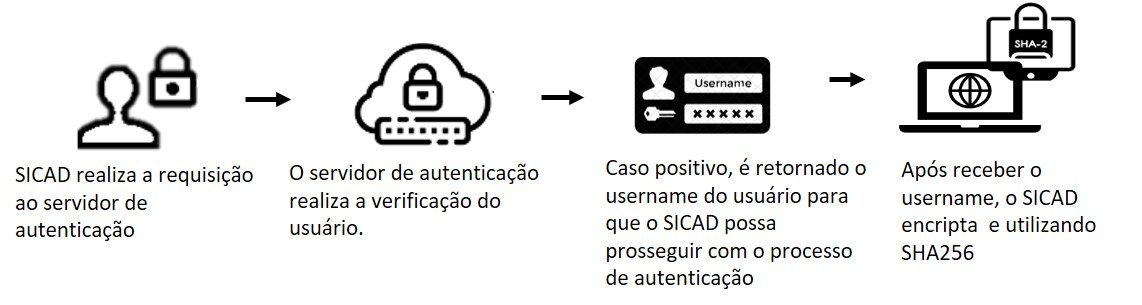
\includegraphics[scale=0.80]{fluxograma_criptografia.jpg}
\caption{Fluxograma do Processo de Criptografia}
\label{fig:processo_autenticacao}
\end{figure}
\par Por conseguinte, com o usuário criptografado a integridade da informação será mantida sendo assim confiável que o usuário a utilize o sistema de forma segura.

\section{ Perfis}
\par
A utilização de perfis de usuários está atrelada a restrição de acesso a funcionalidade do sistema que embora não elimine por completo os riscos à  segurança da informação, diminui em muito a ocorrência de incidentes que comprometam os critérios de confidencialidade, integridade e disponibilidade definidos e exemplificados a seguir.
\begin{itemize}
\item \textbf{Confidencialidade:} um princípio de segurança que requer que dados devam somente ser acessados por pessoas autorizadas;
\item \textbf{Integridade:} um princípio de segurança que garante que dados e itens de configuração somente sejam modificados por pessoas e atividades autorizadas. A integridade considera todas as possíveis causas de modificação, incluindo falhas de hardware e software, eventos ambientais e intervenção humana;
\item \textbf{Disponibilidade:} o princípio de segurança que que garante que a informação que requer que dados devam ser acessados por pessoas autorizadas, no momento que requisitados.
\end{itemize}
\subsection{O controle de Acesso}
O controle de acessos é um processo de segurança essencial que é até mesmo difícil de imaginar como uma organização teria condições de continuar funcionando sem ele. Daí a importância de se estabelecer na organização uma política de controle de acessos, que deve estar de acordo com os requisitos de negócio e de segurança anteriormente definidos.
\subsection{Tipos de controle de acesso}
Essa parte do controle de acesso nas informações da empresa pode basear-se em regras, conforme já mencionamos, bem como em outras diferentes classificações. Dentre os principais tipos de controle que podem ser implantados, podemos destacar os controles de acesso:
\begin{itemize}
\item \textbf{Baseado em perfis}
Também conhecido como Role Based Access Control (RBAC), o acesso é determinado em função de grupos de trabalho (departamentos) ou do próprio cargo exercido pelo usuário. No caso, cada perfil terá seus privilégios aplicados de forma genérica.
\item \textbf{Mandatório (Obrigatório)}
Essa classificação de controle costuma ser representada pelo acrônimo MAC (Mandatory Access Control). Por meio desta funcionalidade, é o sistema quem aplica as políticas de acesso, obedecendo às configurações de privilégio (definidas pelo administrador de sistemas) e a rotulação das informações (feita pelo gestor da informação).
Geralmente, o controle de acesso mandatório é utilizado por empresas que trabalham com dados críticos e sensíveis, ou seja, onde o acesso não autorizado pode acarretar em graves consequências.
\item  \textbf{Discricionário}
No controle de acesso discricionário (Discretionary Access Control – DAC), quem determina as regras e critérios de acesso às informações é o proprietário do recurso. Em poucas palavras, o proprietário da informação define os usuários que podem acessá-la.
Sendo assim, para que esse tipo de controle de acesso nas informações seja implantado corretamente, é necessário que todo e qualquer objeto armazenado no sistema tenha um proprietário e este concederá as permissões de acesso aos devidos usuários.
Criar o controle de acesso nas informações é um grande passo para assegurar a segurança e integridade dos dados contidos no sistema. No entanto, o processo requer um bom planejamento para que seja escolhido o mecanismo adequado para o perfil da empresa.
\end{itemize}

\section{ Moderação}
\section{ Anonimato}
\section{ Segurança}
\section{ Principais Funcionalidades}

%-------------Capítulo 4-----------------
\chapter{Considerações Finais}

%-------------Bibliografia------------------

\renewcommand\bibname{Referências}
\bibliographystyle{unsrt}
\bibliography{referencias}
\nocite{*}

%-------------Apêndice------------------
\appendix

\end{document}
